\documentclass[12 pt, a4paper]{article}

% Текст
\usepackage[utf8]{inputenc} % UTF-8 кодировка
\usepackage[russian]{babel} % Русский язык
\usepackage{indentfirst} % красная строка в первом параграфе в главе
% Отображение страниц
\usepackage{geometry} % размеры листа и отступов
\geometry{
	left=12mm,
	top=25mm,
	right=15mm,
	bottom=17mm,
	marginparsep=0mm,
	marginparwidth=0mm,
	headheight=10mm,
	headsep=7mm,
	nofoot
}
\usepackage{afterpage,fancyhdr} % настройка колонтитулов
%\usepackage{afterpage} % настройка колонтитулов
\pagestyle{fancy}
\fancypagestyle{style}{ % создание нового стиля style
	%\fancyhf{} % очистка колонтитулов
	%\fancyhead[LO, RE]{Обзор на статьи по применнению обучения с подкреплением в робототехнике} % название документа наверху
	%\fancyhead[RO, LE]{\leftmark} % название section наверху
	\fancyfoot[RO, LE]{\thepage} % номер страницы справа внизу на нечетных и слева внизу на четных
	\renewcommand{\headrulewidth}{0pt} % толщина линии сверху
	\renewcommand{\footrulewidth}{0pt} % толцина линии сниз
}
\fancypagestyle{plain}{ % создание нового стиля plain -- полностью пустого
	\fancyhf{}
	\renewcommand{\headrulewidth}{0pt}
\fancyfoot[C]{\thepage} 
}

\addto\captionsrussian{\def\refname{Список используемой литературы}}
% Математика
\usepackage{amsmath, amsfonts, amssymb, amsthm} % Набор пакетов для математических текстов
%\usepackage{dmvnbase} % мехматовский пакет latex-сокращений
\usepackage{cancel} % зачеркивание для сокращений
% Рисунки и фигуры
\usepackage[pdftex]{graphicx} % вставка рисунков
\usepackage{wrapfig, subcaption} % вставка фигур, обтекая текст
\usepackage{caption} % для настройки подписей
%\captionsetup[figure]{name=Рисунок}
%\captionsetup{figurewithin=none,labelsep=period, font={small,it}} % настройка подписей к рисункам
\captionsetup[figure]{figurewithin=none,labelsep=period, font={small,it},name=\text{Рисунок}} % настройка подписей к рисункам
% Рисование
\usepackage{tikz} % рисование
\usepackage{circuitikz}
\usepackage{pgfplots} % графики
% Таблицы
\usepackage{multirow} % объединение строк
\usepackage{multicol} % объединение столбцов
% Остальное
\usepackage[unicode, pdftex]{hyperref} % гиперссылки
\usepackage{enumitem} % нормальное оформление списков
\setlist{itemsep=0.15cm,topsep=0.15cm,parsep=1pt} % настройки списков
% Теоремы, леммы, определения...
\theoremstyle{definition}
\newtheorem{Def}{Определение}
\newtheorem*{Axiom}{Аксиома}
\theoremstyle{plain}
\newtheorem{Th}{Теорема}
\newtheorem{Lem}{Лемма}
\newtheorem{Cor}{Следствие}
\newtheorem{Ex}{Пример}
\theoremstyle{remark}
\newtheorem*{Note}{Замечание}
\newtheorem*{Solution}{Решение}
\newtheorem*{Proof}{Доказательство}
% Свои команды
\newcommand{\comb}[1]{\left[\hspace{-4pt}\begin{array}{l}#1\end{array}\right.\hspace{-5pt} } % совокупность уравнений
% Титульный лист
\usepackage{csvsimple-l3}
\title{\large{Обзор на статьи по применению обучения с подкреплением в робототехнике}}
\author{А.~А. Нечаева \\ E-mail: \href{mailto:anechaeva142@gmail.com}{ anechaeva142@gmail.com}
 \and  К.~О. Велюго \\ E-mail: \href{mailto:kirillvelyugo@ya.ru}{kirillvelyugo@ya.ru} 
\and А.~К. Иванов   \\ E-mail: \href{mailto:Edelwiw@gmail.com}{Edelwiw@gmail.com} 
 \and А.~А.  Воротников  \\ E-mail: \href{mailto:vorotnikovandrej46@gmail.com}{vorotnikovandrej46@gmail.com} 
 \and А.~И. Сон  \\ E-mail: \href{mailto:sunnnya@mail.ru}{sunnnya@mail.ru} }
\date{}

\begin{document}
\maketitle
\pagestyle{plain}
\begin{abstract}
Данная работа посвящена обзору 6 статей, в которых описаны различные случаи применения обучения с подкреплением для решения задач робототехники. В обзоре уделено особое внимание содержащимся в изученненных источниках предложениям по усовершенствованию обучения с подкреплением, оптимизации алгоритмов для повышения эффективности процесса обучения. 
\end{abstract}
\section{Введение}
Обучение с подкреплением (англ.\textit{reinforcement learning}) -- один из способов машинного обучения, в котором испытуемая система (агент) обучается, взаимодействуя с некоторой средой. \\
Основные элементы RL системы:\\
-- агент (обучающийся);\\
-- среда, с которой агент взаимодействует в процессе обучения;\\
-- действие агента, которое следует заданной стратегии;\\
-- награда, которую агент получает в зависимости от успешности выполнения определенного действия.\\
Условную последовательность взаимодействия компонентов системы в процессе обучения иллюстрирует рисунок (\ref{ris:1}).
\begin{figure}[h]
		\begin{center}
                      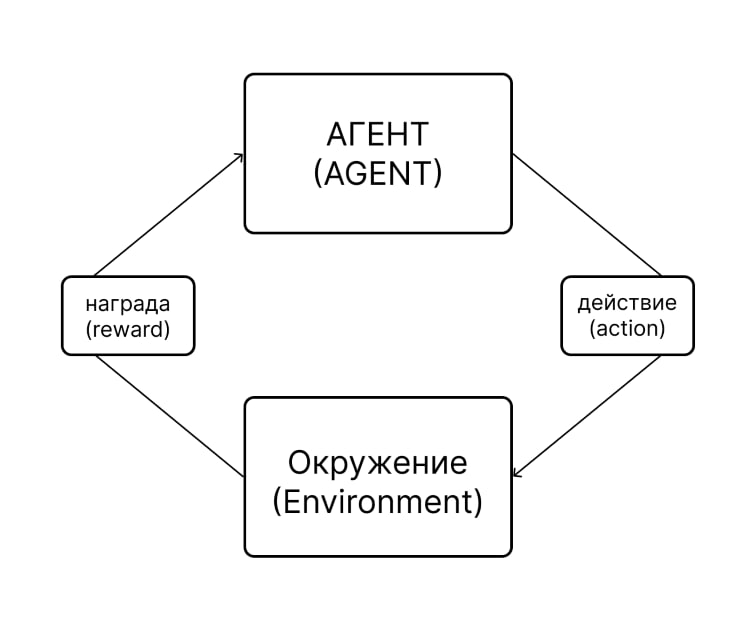
\includegraphics[scale=0.5]{"./РЛ_компоненты.jpg"}
	           \caption{Компоненты системы обучения с подкреплением}\label{ris:1}
		\end{center}
\end{figure}\\
В основе выбора наиболее оптимальной стратегии поведения агента в среде используется Марковский процесс принятия решений (рисунок (\ref{ris:2})), в котором существует 3 основных параметра:\\
-- S -- конечное множество состояний;\\
-- A -- конечное множество действий;\\
-- R -- вознаграждение.\\
Вознаграждение является функцией, зависящей от начального состояния агента $s$, действия $a$, которое он совершил для перехода в состояние $s'$. И записывается: $R_a (s, s')$.

\begin{figure}[h]
		\begin{center}
                      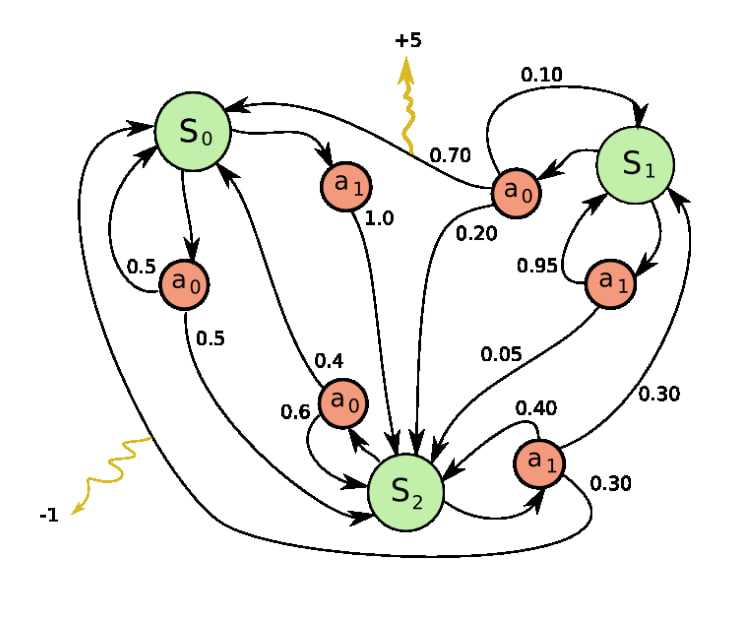
\includegraphics[scale=0.5]{"./мппр.jpg"}
	           \caption{Марковский процесс принятия решений}\label{ris:2}
		\end{center}
\end{figure}
Вероятность того, что действие $a$ при состоянии $s$ во время $t$ приведет в состояние $s'$ ко времени $t+1$ выражается формулой( \ref{eq2}).
\begin{equation}\label{eq2}
P_a(s, s') = Pr(s_{t+1} = s' | s_t = a, \, a_t = a)
\end{equation}

Принципы, на которых базируется метод обучения с подкреплением:\\
-- агенту известна конечная цель, но не алгоритм ее достижения;\\
-- обучение происходит путем проб и ошибок;\\
-- системе заранее неизвестны правильные действия;\\
-- цель RL -- обучить агента определенному поведению.\\

В произвольный момент времени t агент характеризуется состоянием $s_t \in S$ и набором возможных действий 
$A(s_t)$. После выбора определенного действия $a \in A(s_t)$, он переходит в состояние $s_{t+1}$ и получает выигрыш $r_t$. Основываясь на таком взаимодействии с окружающей средой, агент, обучающийся с подкреплением, должен выработать стратегию $\pi: S \to A$, которая максимизирует величину $R$, которую можно выразить формулой (\ref{eq1}).
\begin{equation}\label{eq1}
R = \sum \gamma^t r^t,
\end{equation}
где $\gamma \in [0;1]$. Величины могут быть различными.
Задача агента --  максимизировать вознаграждение за минимальное время.\\
На основе получаемого вознаграждения агент формирует функцию полезности $Q$, что впоследствии предоставляет ему возможность не случайно выбирать стратегию поведения, а учитывать опыт прошлых взаимодействий со средой. Наглядно процесс можно представить, используя таблицу со всевозможными парами состояний / действий для более эффективного выбора. Пример подобной таблицы изображен на рисунке (\ref{ris:3}).\cite{litlink1}
\begin{figure}[h]
		\center{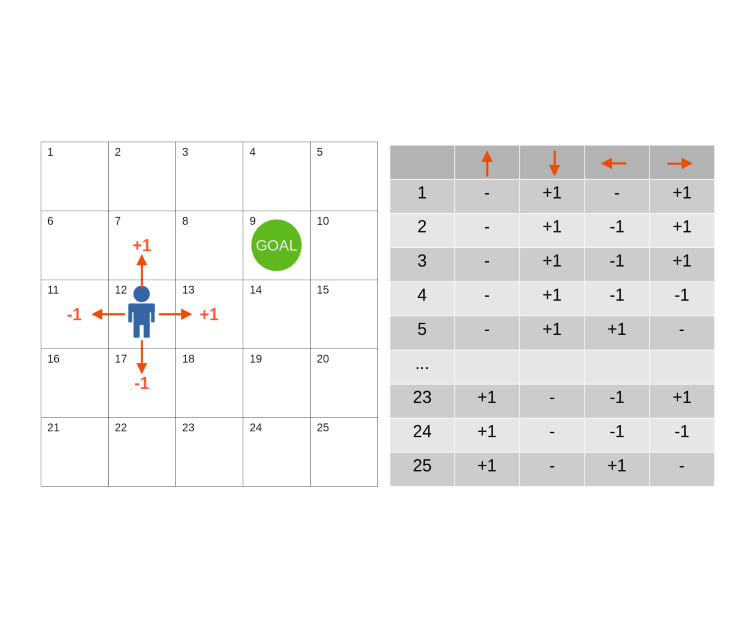
\includegraphics[width=1\linewidth]{"./Q-table.jpg"}}
                    %  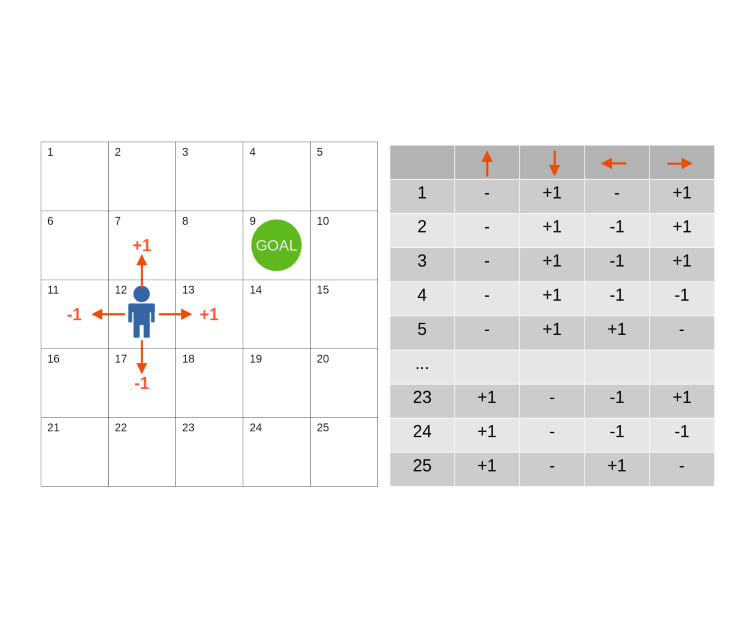
\includegraphics{"./Q-table.jpg"}
	           \caption{Q-таблица}
		
\label{ris:3}
\end{figure}
К преимуществам обучения с подкреплением можно отнести фокусировку на проблеме в целом, отсутствие необходимости  в этапе сбора данных, способность подстраиваться под динамичные и новые среды. У данного метода машинного обучения также есть и недостатки, например, большое количество времени на обучение и отсуствие возможности повлиять на принимаемые агентом решения.
\\\\\\
\section{Применение обучения с подкреплением в робототехнике}
\subsection{Метод самопроверки электростанций с помощью беспилотных летательных аппаратов с использованием глубокого Q-сетевого обучения с подкреплением \cite{litlink2}}

Целью ученых было обследование производственных предприятий, в том числе электростанций, по-прежнему довольно опасно для людей, так может произойти несчастный случай, также это требует специальной подготовки людей. Поэтому проще становится использовать БПЛА для инспекции электростанций.\\
Для навигации БПЛА необходимо учитывать не только внутренние факторы, но и влияние окружающей среды. Все это можно учесть с помощью алгоритмов RL. Что касается традиционных методов навигации, они менее гибкие и требуют больших затрат при использовании датчиков.\\

Навигация БПЛА во время инспекции является основной темой данной работы. Электростанция, содержащая здания и провода, является местом проведения инспекции. Модель используется для изображения электростанции, а также внутренних и внешних условий окружающей среды, включая количество ветра и уровень заряда, среди прочего.\\

Общее вознаграждение дрона может быть вычислено путем сложения вознаграждения  за подъем и вознаграждения за достижение цели. Однако некоторые дополнительные вознаграждения и наказания предоставляются на различных этапах завершения, например, при завершении полета в точке цели со столкновением или разряд аккумулятора без столкновения и т. д. Эти этапы завершения рассматриваются с каждой соответствующей модификацией вознаграждения. В данном случае избежание столкновений имеет первостепенное значение.\\

По результатам эксперимента после 40000 эпизодов обучения, предварительно обученная модель достигла своего потолка и набранный результат стал уменьшаться, поэтому обучение было приостановлено. \\
При сравнении предварительно обученной модели с финальной, результат заметен, так как последняя полностью избегает столкновений, что не удается первой. Результаты испытаний предварительно обученной модели представлены на рисунке (\ref{ris:4}), модель полученная учеными в конце эксперимента демонстрирует траекторию изображенную на рисунке (\ref{ris:5})\\

\begin{figure}[h]
		\center{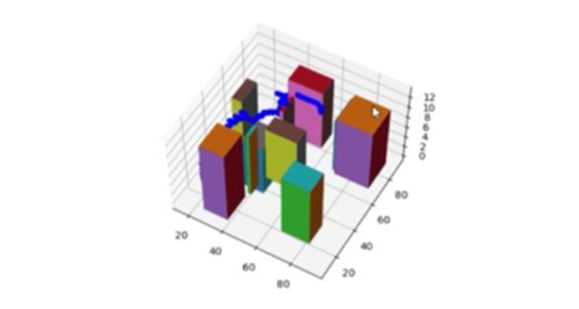
\includegraphics[width=0.5\linewidth]{"./андрей1.jpg"}}
                    %  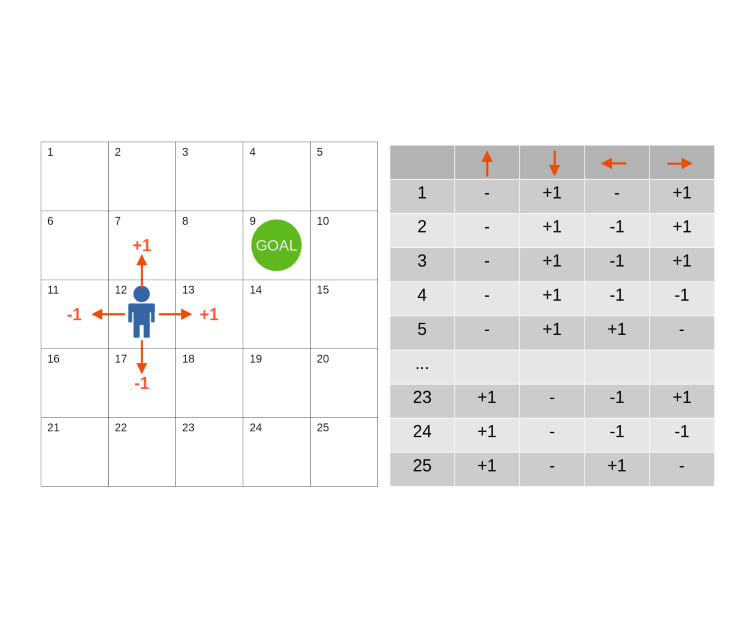
\includegraphics{"./Q-table.jpg"}
	           \caption{Траектория движения предобученной модели в виртуальной среде}
		
\label{ris:4}
\end{figure}

\begin{figure}[h]
		\center{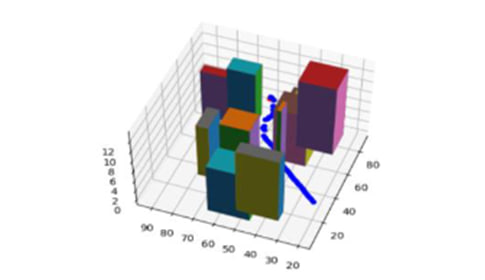
\includegraphics[width=0.5\linewidth]{"./андрей2.jpg"}}
                    %  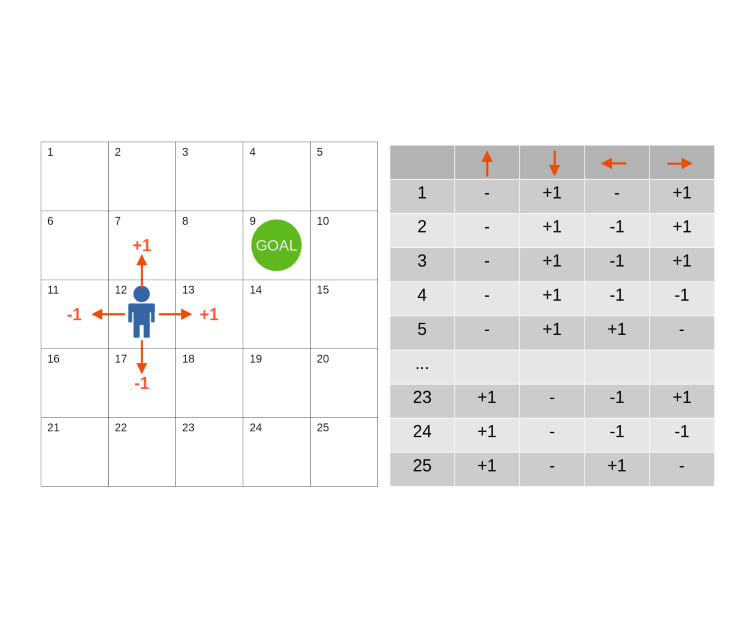
\includegraphics{"./Q-table.jpg"}
	           \caption{Траектория движения финальной модели в виртуальной среде}
		
\label{ris:5}
\end{figure}


Стратегия, описанная в исследовании, использует метод обучения с подкреплением DQN, чтобы научить БПЛА учиться ориентироваться в случайно сгенерированном месте модели электростанции, которая учитывают как внутренние, так и внешние факторы.\\
Моделирование результатов демонстрирует, что этот метод может предложить БПЛА шаблон для навигации в намеченное место, сохраняя при этом осведомленность о себе и своем окружении. График результатов результатов обучения подтверждает правильность методики эксперимента.\\


\subsection{Автономная посадка дрона на движущиеся платформы, основывающаяся на обучении с подкреплением \cite{litlink3}}
Целью работы ученых было создание алгоритма управления многомоторными беспилотными летательными аппаратами (БПЛА) на основе глубокого обучения с подкреплением, который сможет обеспечивать посадку на подвижную платформу для пополнения заряда батарей и выгрузки данных. Экспериментальную установку можно увидеть на рисуноке(\ref{ris:6}).\\

Классические подходы решения данной задачи основаны на сложных моделях взаимодействия БПЛА с окружающей средой, для вывода которых требуется потратить огромное количество усилий. Использование обучения с подкреплением предлагает альтернативу создания точных моделей — обучение алгоритма управления на данных, полученных исключительно во время процедуры тренировки, что многократно упрощает задачу создания подобных алгоритмов. \\

Для решения данной задачи авторы статьи проходят несколько этапов, которые представляют собой упрощенные, но сильно схожие с начальной задачи. \\

Несмотря на плюсы подобного решения, алгоритмы глубокого обучения очень чувствительны к постановке задачи, это может привести к длительному обучению и необходимости подбора гиперпараметров путем проб и ошибок. Кроме того, глубокая нейронная сеть действует как черный ящик — невозможность определить, что именно привело систему к такому поведению накладывает определенные трудности в разработке подобных алгоритмов. \\

\begin{figure}[h]
		\center{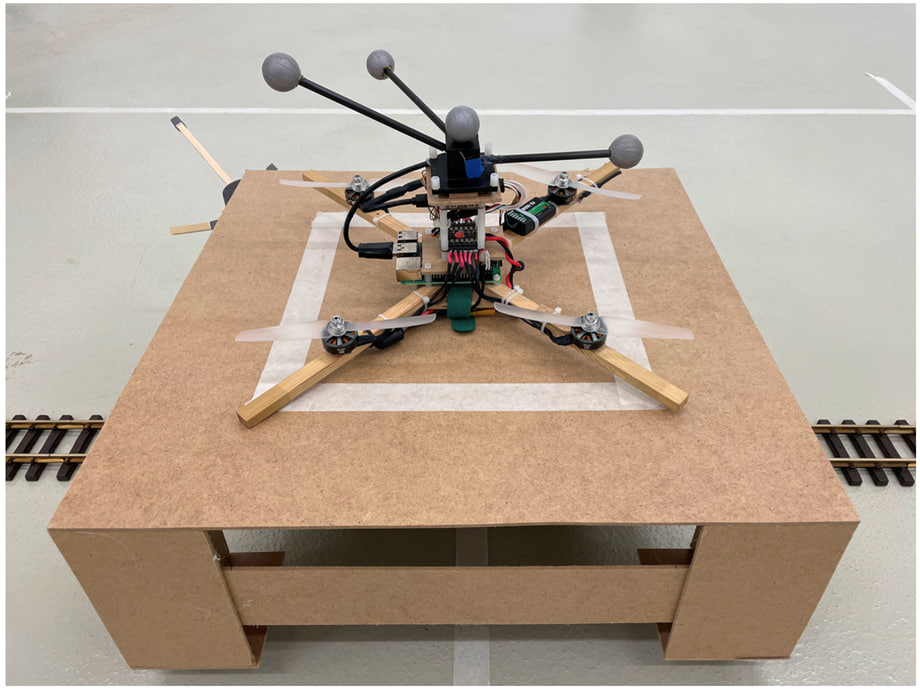
\includegraphics[width=1\linewidth]{"./бпла.jpg"}}
                    %  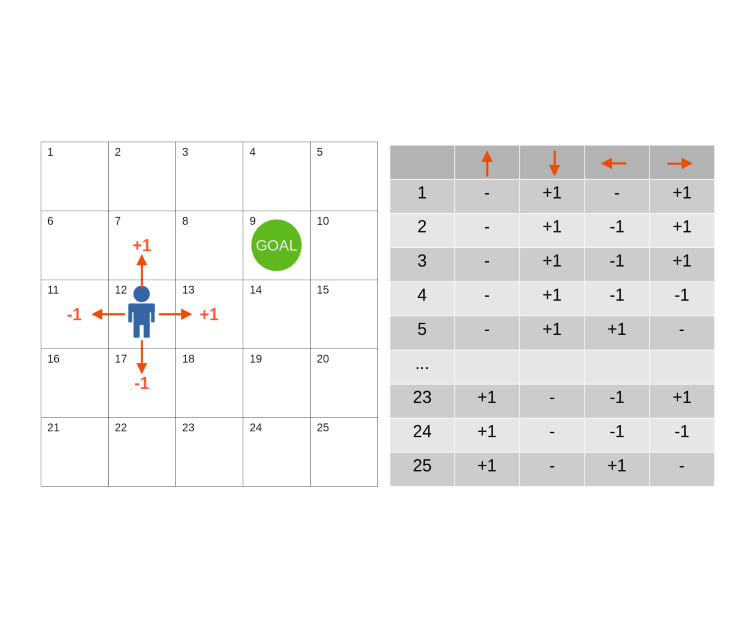
\includegraphics{"./Q-table.jpg"}
	           \caption{Дрон с подвижной платформой, на которую он должен сесть}
		
\label{ris:6}
\end{figure}
Для достижения цели авторами было решено использовать табличный алгоритм Q-learning. Использование этого метода не требует испльзование мощного графического процессора для обучения, что дает возможность производить использовать алгоритм на вычислительных мощностях бортового компьютера БПЛА. \\

Использование алгоритмы глубокого обучения, кроме прочего, позволяет оптимизировать “действие-ценность”, что приводит к оптимальному выбору действий. \\

Ход работы: \\
Авторы разделил тренировку алгоритма на несколько этапов:\\
1.	Компьютерное моделирование процессов в среде Gazebo 11 без “шумов” — для начальной тренировки алгоритма. \\
2.	Моделирование в условиях, приближенных к реальным. Шумы от датчиков, влияние среды и тд. \\
3.	Тесты на реальных БПЛА — для окончательной тренировки алгоритма и проверки его в реальных условиях. \\

Для выполнения каждого из шагов тренировки использовался мощный ПК. \\
В результате работы, авторам статьи удалось создать рабочий алгоритм управления БПЛА для посадки на подвижную платформу, движущуюся в одном измерении (по горизонтали). \\

\subsection{Обучение роботов подражать движениям животных \cite{litlink4}}
При сотрудничестве c Google Brain исследователи попытались выяснить возможно ли создавать роботов с меньшими ресурсами разработки, подражая настоящим животным.\\

Исследование было актуально тем, что разработка контроллеров, позволяющих роботам воспроизводить движения животных (ходьба вперед, назад, разворот) часто является сложной задачей. Возможность обучать роботов на примере животных существенно смогла бы упростить и удешевить процесс разработки.\\
Для обучения был использован робот Laikago. Сперва был записан видеоролик, где показаны основные движения животного (для примера была взята собака). Система использовала обучение с подкреплением для обучения политики управления, которая позволяет роботу имитировать движение животного. Агенты сначала обучались в симуляции, а затем, были перенесены в реальный мир с помощью техники адаптации латентного пространства, которая позволяет эффективно адаптировать политику обучения. \\
Система состоит из трех основных элементов: ретаргетинг движения, имитация движения и адаптация.
Сначала, учитывая исходные движения животного, этап ретаргетинга движения сопоставляет движение с морфологией исходного животного и робота.
Затем этап имитации движения использует ретаргетированное движение для обучения агента в симуляции
Наконец, на этапе адаптации результат работы симуляции переносится на реального робота, рисунок(\ref{ris:7}) .\\

\begin{figure}[h]
		\center{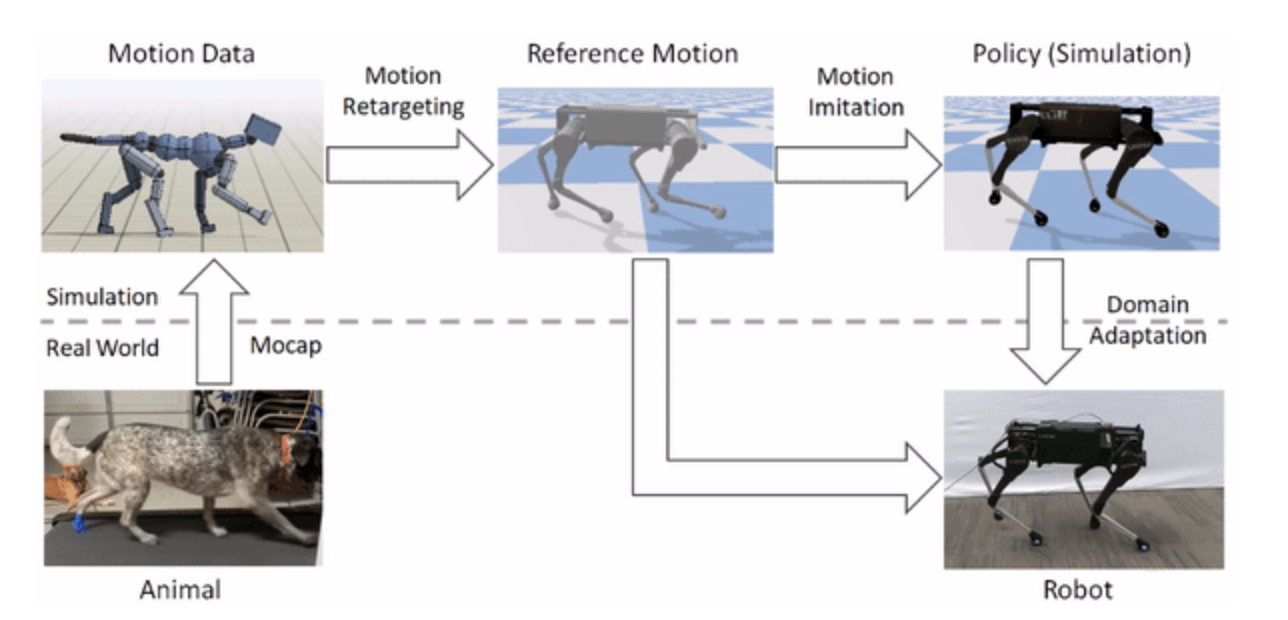
\includegraphics[width=1\linewidth]{"./вел1.png"}}
                    %  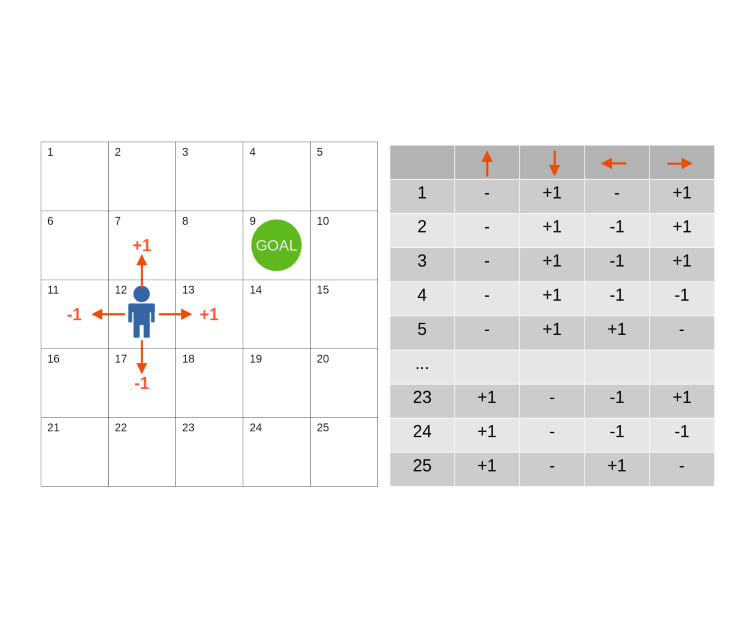
\includegraphics{"./Q-table.jpg"}
	           \caption{Этапы работы фреймворка}
		
\label{ris:7}
\end{figure}

Ретаргетинг движения. Цель этого этапа является создание эталонного движения для робота, которое отражает важные характеристики движения животного. Для этого определяют набор исходных ключевых точек на теле животного (бедра, ступни). Аналогичную операцию производят с телом робота, рисунок (\ref{ris:8}). \\
\begin{figure}[h]
		\center{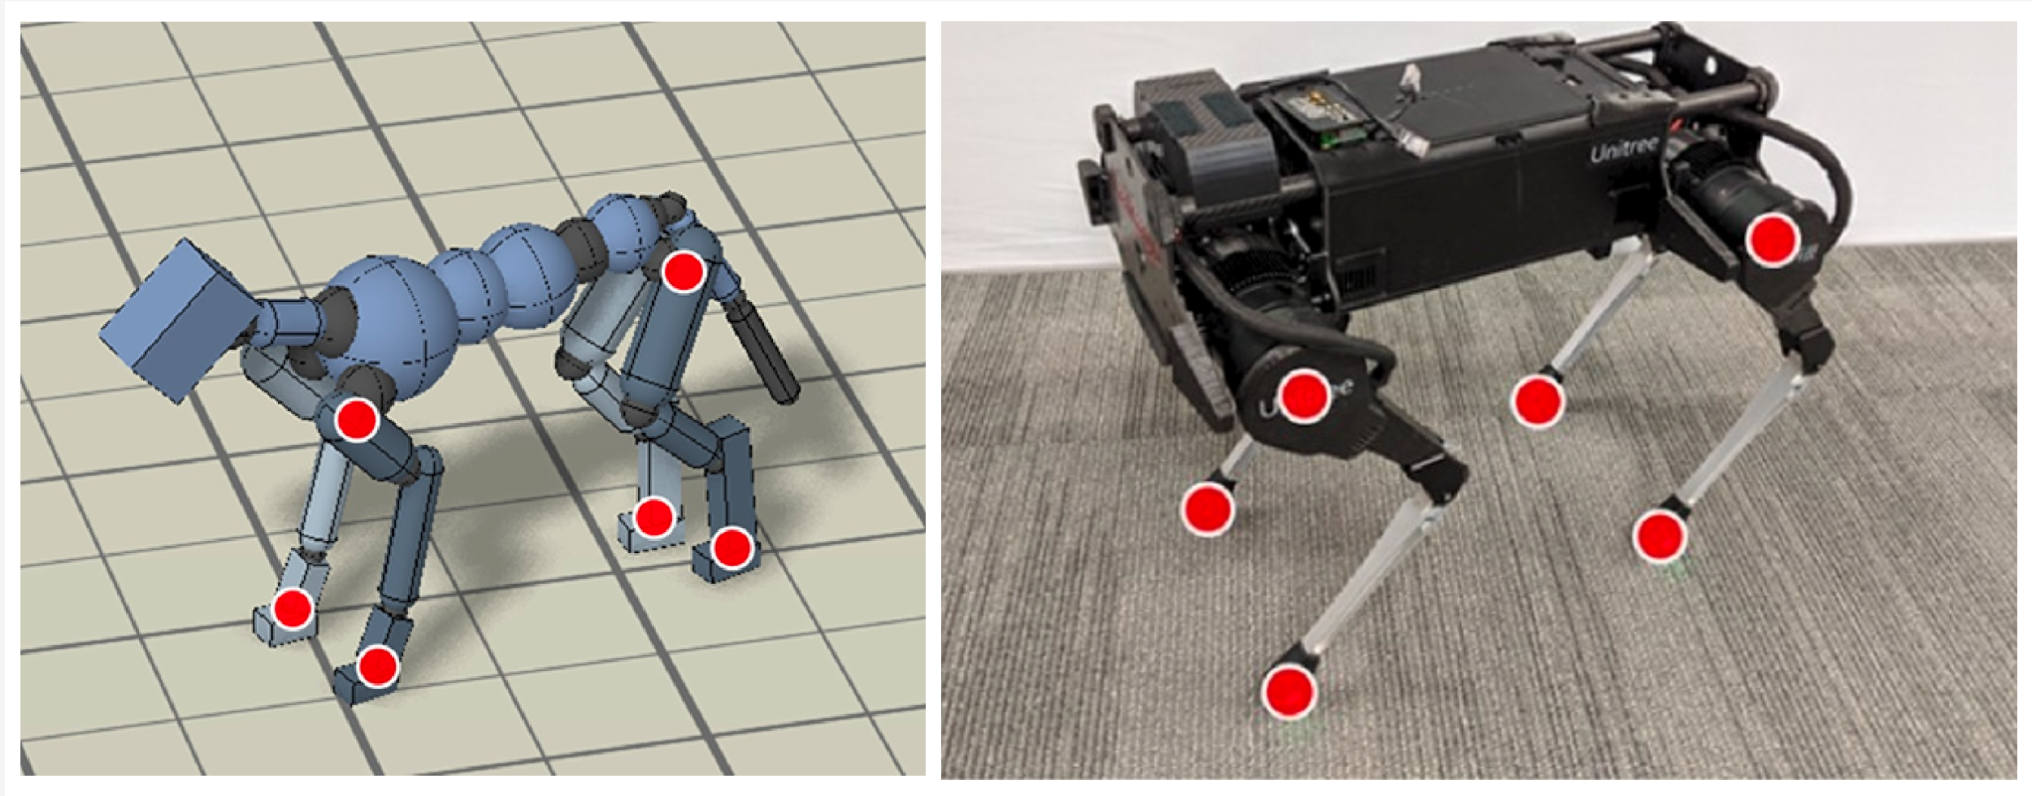
\includegraphics[width=1\linewidth]{"./вел2.png"}}
                    %  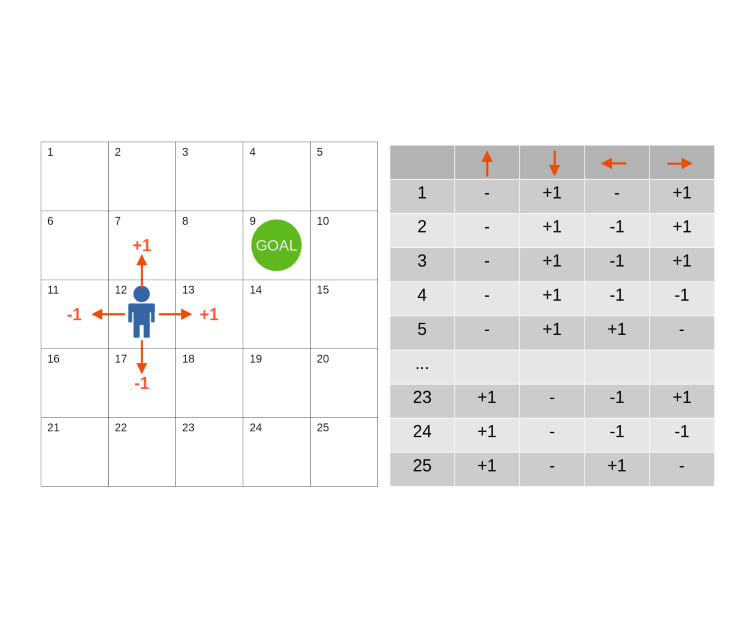
\includegraphics{"./Q-table.jpg"}
	           \caption{Ретаргетинг движения}
		
\label{ris:8}
\end{figure}
Имитация движения. Для этого этапа сначала использовали симуляцию с  помощью PyBullet. После получения первичной политики ее перенесли в реальный мир, используя эффективные методы адаптации. \\
В процессе обучения была использована следующая политика п(a|s, g). Она принимает состояние s (конфигурацию тела робота), цель g (определена целевыми позами из эталонного движения, которые робот должен имитировать). Затем робот выдает действие a, которое задает целевые углы для PD регуляторов на каждом из суставов робота. \\
Для обучения была использована система вознаграждений, которая мотивировала агента минимизировать разницу между эталонным движением q' и движением в симуляции q на каждом временном интервале t .\\

Адаптация. Для переноса политики из симуляции в реальный мир были использованы эффективные методы адаптации, которые позволяют адаптировать политику к реальному миру, используя лишь небольшое количество испытаний на реальном роботе.\\
В итоге исследователи получили следующее: система способна обучить робота имитировать различные навыки животного. Также были сравнены политики с разработанными вручную контроллерами — политики, использовавшие обучение с подкреплением, оказались способны к более быстрому обучению. Но из-за аппаратных и алгоритмических ограничений команде исследователей не удалось имитировать более динамичные движения. Выученные политики не является абсолютно надежными, сравнивая с лучшими контроллерами, которым были разработаны вручную.




\subsection{Обучение с подкреплением в задаче манипулирования различными объектами на основе визуальной информации \cite{litlink5}}
Научные сотрудники из лаборатории моделирования, Samsung Research, Samsung Electronics, задались целью предложить новую структуру обучения с подкреплением AP-NPQL (Non-Parametric Q Learning with Action Primitieves) и оценить ее эффективность, применительно к манипуляторам, получающих информацию об окружающем мире через камеры. 
Задачи манипулирования, на которых проводилось тестирование алгоритма: толкание тарелки, укладка коробок, переворачивание чашки, захват и размещение тарелки – актуальные задачи, например, для робота, занимающегося работой по дому.\\
Обучение с подкреплением актуально в данном случае, потому что на основе визуальных данных робот должен определить, какой объект нужно взять, где его схватить, где и как поставить. \\
Однако у RL есть недостатки, например, низкая выборка и ошибочные «оптимальные» стратегии (последние вызваны попаданием в локальные оптимумы при использовании метода градиентного спуска). Все это усложняется высокой размерностью визуального ввода.\\
В качестве усовершенствования алгоритма обучения с подкреплением предлагается упрощение параметрической части алгоритма и введения набора примитивов действий.

\subsection{Исследование алгоритмов повышающих качество обучения с подкреплением в симуляции для использования на реальных робототехнических системах  \cite{litlink6}}

Целью ученых было решение проблемы с поиском наиболее результативного метода машинного обучения, которая возникает в связи с проблемой применимости экспериментов в реальной среде (влияние шумов измерений, погрешностей, невозможности полного переноса модели окружения и агента в симуляцию и тд.). Для этого появилась область задач sim-to-real, в методы которой входят Domain Randomization and Adaptation, Transfer Learning, Meta Learning.\\

Поиск лучшего метода действительно является актуальным вопросом в наше время, решение которого и затрагивается в данной статье. Суть заключается в том, что вышеуказанные методы как раз учитывают те же самые шумы сигналов датчиков состояний, в архитектуру добавляются новые агенты, выполняются разбиения на меньшие по размерности задачи. В исследовании более подробно речь идет о Domain Randomization и Meta Learning, а также о Meta Strategy Optimization. \\

Их основная цель заключается в улучшении устойчивости и обобщающей способности модели, путем предъявления ей широкого спектра синтетических или искуственно созданных обучающих данных. За счёт этого модель становится более адаптивной и способной справляться с различными реальными сценариями.\\

Для того, чтобы протестировать вышеупомянутые алгоритмы была выбрана задача передвижения четырехногого робота по сложной поверхности. Речь идет о неоднородной поверхности, имеющей уклоны, перепады высот, неровности и тд. Использовался физический симулятор PyBullet, а системе были доступны измерения одометрии робота (речь идет о положении лап относительно системы координат тела, измерениях датчиков инерциального блока в теле робота), угловой и линейной скорости лап, измерения датчика касания поверхности. \\


\subsection{Применение алгоритма DDPG обучения с подкреплением для мобильного робота \cite{litlink7}}
Целью ученых было сравнение алгоритма обучения с подкреплением (c DQN) с алгоритмом с двумя критиками на примере виртуальной модели мобильного робота. Модель имеет датчик цвета и должна ехать максимально близко к цветоконтрастной линии со скоростью 1м/с. \\
Цель алгоритма найти значения коэффициентов для ПИД-регулятора.\\
Полученные коэффициенты показывают, что оба алгоритма достигают поставленной цели - скорости движения 1м/с. Однако алгоритм DDPG (основанные на обучении с подкреплением) позволяет агенту сделать это быстрее.


\section{Заключение}
Обучение с подкреплением находится на заре своего развития, хотя уже к сегодняшнему времени ученым удалось достичь значительных успехов в применении и совершенствовании его алгоритмов. Например, в задачах управления беспилотными летательными аппаратами ученым удалось улучшить результальты и точность траектории полета. Поиск решений некоторых задач с помощью существующих алгоритмов обучения с подкреплением оказывается сложным из-за особенностей систем, математических аспектов и большого объема времени, затрачиваемого на процесс обучения. Однако у обучения с подкреплением существует огромный потенциал для будущего развития: алгоритмы будут совершенствоваться, а вычислительные мощности техники будут возрастать, что сократит временные затраты на обучение.

\newpage
\addcontentsline{toc}{section}{Список литературы}
%далее сам список используевой литературы
\begin{thebibliography}{}
    \bibitem{litlink1}  Corentin Risselin  -  Understanding Q-learning: How a Reward Is All You Need
    \bibitem{litlink2}   Haoran Guan  -  Self-Inspection Method of Unmanned Aerial Vehicles in Power Plants Using Deep Q-Network Reinforcement Learning
    \bibitem{litlink3}  Pascal Goldschmid and Aamir Ahmad  -  Reinforcement Learning based Autonomous Multi-Rotor Landing on Moving Platforms
    \bibitem{litlink4}  Xue Bin (Jason) Peng  -  Robots Learning to Move like Animals
    \bibitem{litlink5}  Dongwon Son, Myungsin Kim, Jaecheol Sim, and Wonsik Shin  -  Reinforcement Learning for Vision-based Object Manipulation with Non-parametric Policy and Action Primitives 
    \bibitem{litlink6}  Труфанова А.А., Симонов Р.А., Симонов Н.А. (науч. рук. Ведяков А.А.).   -  Исследование алгоритмов повышающих качество обучения с подкреплением в симуляции для использования на реальных робототехнических системах
    \bibitem{litlink7}  Т. Ю. Ким  -  Применение алгоритма DDPG обучения с подкреплением для мобильного робота
 
\end{thebibliography}
 


\end{document}













